\documentclass[11pt,a4paper]{report}
% ====================================================================
% PRÉAMBULE — moteur XeLaTeX (tectonic)
% ====================================================================
\usepackage{fontspec}
% police principale = Latin Modern par défaut de fontspec (pas besoin de la nommer)
\setsansfont{DejaVu Sans}
\setmonofont{DejaVu Sans Mono}[Scale=0.85]

\usepackage{polyglossia}
\setdefaultlanguage{french}
% guillemets français (non fournis par polyglossia)
\providecommand{\og}{«\,}
\providecommand{\fg}{\,»}

\usepackage{geometry}
\geometry{a4paper,margin=2.3cm,headheight=15pt}

\usepackage{amsmath,amssymb}
\usepackage{graphicx}
\usepackage{booktabs}
\usepackage{array}
\usepackage{multirow}
\usepackage{enumitem}
\usepackage{caption}
\captionsetup{font=small,labelfont=bf}

\usepackage[table]{xcolor}
% --- palette ---
\definecolor{bleu}{HTML}{2C3E72}
\definecolor{bleuclair}{HTML}{4C72B0}
\definecolor{vert}{HTML}{2E7D32}
\definecolor{vertclair}{HTML}{E8F5E9}
\definecolor{rouge}{HTML}{C0392B}
\definecolor{rougeclair}{HTML}{FDEDEC}
\definecolor{orange}{HTML}{E67E22}
\definecolor{orangeclair}{HTML}{FEF5E7}
\definecolor{violet}{HTML}{6C3483}
\definecolor{violetclair}{HTML}{F4ECF7}
\definecolor{gristresclair}{HTML}{F5F5F5}
\definecolor{griscode}{HTML}{2B2B2B}

% --- code Python ---
\usepackage{listings}
\definecolor{cmt}{HTML}{6A9955}
\definecolor{kw}{HTML}{569CD6}
\definecolor{str}{HTML}{CE9178}
\definecolor{num}{HTML}{B5CEA8}
\lstdefinestyle{py}{
  language=Python,
  basicstyle=\ttfamily\footnotesize,
  keywordstyle=\color{kw}\bfseries,
  commentstyle=\color{cmt}\itshape,
  stringstyle=\color{str},
  numberstyle=\tiny\color{gray},
  numbers=left,numbersep=7pt,
  backgroundcolor=\color{gristresclair},
  frame=leftline,framerule=2pt,rulecolor=\color{bleuclair},
  breaklines=true,breakatwhitespace=true,
  showstringspaces=false,
  tabsize=4,
  upquote=true,
  columns=fullflexible,keepspaces=true,
  literate=%
    {é}{{\'e}}1 {è}{{\`e}}1 {ê}{{\^e}}1 {ë}{{\¨e}}1
    {à}{{\`a}}1 {â}{{\^a}}1 {î}{{\^i}}1 {ï}{{\¨i}}1
    {ô}{{\^o}}1 {ö}{{\¨o}}1 {û}{{\^u}}1 {ù}{{\`u}}1 {ç}{{\c c}}1
    {œ}{{\oe}}1 {Œ}{{\OE}}1 {’}{{'}}1
    {É}{{\'E}}1 {È}{{\`E}}1 {Ê}{{\^E}}1 {À}{{\`A}}1
    {≤}{{$\leq$}}1 {≥}{{$\geq$}}1 {²}{{$^2$}}1 {→}{{$\rightarrow$}}1
    {≈}{{$\approx$}}1 {μ}{{$\mu$}}1 {≠}{{$\neq$}}1 {∈}{{$\in$}}1
    {├}{{|}}1 {└}{{|}}1 {─}{{-}}1 {│}{{|}}1 {’}{{'}}1 {«}{{<<}}1 {»}{{>>}}1
}
\lstset{style=py}

% --- boîtes colorées (tcolorbox) ---
\usepackage[most]{tcolorbox}
\tcbset{
  boxedstyle/.style={
    enhanced,breakable,boxrule=0pt,
    leftrule=3pt,arc=2pt,left=8pt,right=8pt,top=6pt,bottom=6pt,
    fonttitle=\bfseries,coltitle=white,
  }
}
\newtcolorbox{Definition}[1][]{boxedstyle,colback=violetclair,colframe=violet,
  title={\faIcon~Définition #1}}
\newtcolorbox{Exemple}[1][]{boxedstyle,colback=vertclair,colframe=vert,
  title={Exemple — #1}}
\newtcolorbox{Calcul}[1][]{boxedstyle,colback=gristresclair,colframe=bleuclair,
  title={Calcul détaillé #1}}
\newtcolorbox{Astuce}[1][]{boxedstyle,colback=orangeclair,colframe=orange,
  title={Astuce / À retenir #1}}
\newtcolorbox{Attention}[1][]{boxedstyle,colback=rougeclair,colframe=rouge,
  title={Attention #1}}
\newtcolorbox{Resume}[1][]{boxedstyle,colback=vertclair,colframe=vert,
  title={En résumé #1}}

% remplace \faIcon si fontawesome absent
\providecommand{\faIcon}[1]{}

% --- titres & en-têtes ---
\usepackage{titlesec}
\titleformat{\chapter}[display]
  {\normalfont\huge\bfseries\color{bleu}}
  {\filright\Large\color{bleuclair}Chapitre~\thechapter}{8pt}{\Huge}
\titlespacing*{\chapter}{0pt}{-20pt}{20pt}

\usepackage{fancyhdr}
\pagestyle{fancy}
\fancyhf{}
\fancyhead[L]{\small\color{bleu}\leftmark}
\fancyhead[R]{\small\thepage}
\renewcommand{\headrulewidth}{0.6pt}

\usepackage{hyperref}
\hypersetup{
  colorlinks=true,linkcolor=bleu,urlcolor=bleuclair,
  citecolor=vert,pdftitle={Cours de Data Mining — Explications complètes},
  pdfauthor={Master 2 IG/ID — ENEAM/UAC}
}

% --- commandes pratiques ---
\newcommand{\gini}{\textit{Gini}}
\newcommand{\R}{\mathbb{R}}


\begin{document}

% ============================ PAGE DE TITRE ============================
\begin{titlepage}
\centering
\vspace*{1.5cm}
{\Large\scshape Université d'Abomey-Calavi — ENEAM\par}
{\large Master 2 — Informatique de Gestion / Ingénierie des Données\par}
\vspace{2.2cm}
{\color{bleuclair}\rule{\linewidth}{2pt}}\par
\vspace{0.8cm}
{\Huge\bfseries\color{bleu} DATA MINING\par}
\vspace{0.5cm}
{\LARGE Cours expliqué pas à pas\par}
\vspace{0.3cm}
{\large Tous les exemples résolus en détail \textbullet{} scripts Python \textbullet{} projet Streamlit\par}
\vspace{0.8cm}
{\color{bleuclair}\rule{\linewidth}{2pt}}\par
\vspace{2.5cm}
\begin{tabular}{rl}
\textbf{Enseignant} & Th. K. DAGBA\\[4pt]
\textbf{Année} & 2025--2026\\[4pt]
\textbf{Contenu} & Chap. 1, 2, 4, 5 + TP classification + Projet\\
\end{tabular}
\vfill
{\small Document compilé avec \texttt{tectonic} (XeLaTeX).\par}
\end{titlepage}

\tableofcontents
\clearpage

% ============================ INTRODUCTION ============================
\chapter*{Mode d'emploi de ce document}
\addcontentsline{toc}{chapter}{Mode d'emploi de ce document}

Ce document reprend \textbf{l'intégralité} du cours de Data Mining et l'explique
\textbf{de la façon la plus simple possible}. Pour chaque chapitre tu trouveras :

\begin{itemize}[leftmargin=1.4em]
  \item la \textbf{théorie} reformulée en mots simples, avec des encadrés colorés ;
  \item \textbf{tous les exemples du cours résolus à la main}, chaque calcul détaillé ;
  \item le \textbf{script Python équivalent} (commenté ligne à ligne) qui refait le
        calcul puis le \textbf{vérifie avec scikit-learn} ;
  \item des \textbf{figures} générées par ces scripts.
\end{itemize}

\begin{Astuce}
Les codes des encadrés \og listing \fg{} sont les vrais fichiers du dossier
\texttt{scripts/}. Tu peux les exécuter avec, par exemple :
\begin{center}\ttfamily uv run python scripts/knn\_david.py\end{center}
Et l'application du projet avec : \ttfamily uv run streamlit run projet/app.py
\end{Astuce}

\begin{Resume}[: les 4 idées clés]
\textbf{1.} Le Data Mining transforme des \emph{données} en \emph{connaissances} pour
\emph{décider}.\quad
\textbf{2.} Quatre tâches : \emph{classification}, \emph{prédiction}, \emph{association},
\emph{segmentation}.\quad
\textbf{3.} \emph{Supervisé} (classe connue) vs \emph{non supervisé} (classe inconnue).\quad
\textbf{4.} 60\,\% du travail = \emph{préparer les données}.
\end{Resume}

% ============================ CHAPITRES ============================
\chapter{Introduction au Data Mining}

\section{Pourquoi le Data Mining ? (motivations)}

\begin{Exemple}[le banquier]
Un client demande un crédit. Le banquier veut savoir \emph{s'il va rembourser}. Le client
ne dira jamais \og je ne rembourserai pas \fg{}. Mais le banquier peut \textbf{inférer} le
comportement futur du client à partir de la \textbf{base de données des anciens clients}.
\textbf{C'est exactement ça le Data Mining} : utiliser le passé (les données) pour prédire/
comprendre le futur.
\end{Exemple}

On vit une \textbf{explosion des données} : bases de données, entrepôts, capteurs,
web, e-commerce, hôpitaux, supermarchés… On produit des téraoctets chaque jour, mais
\textbf{seule une infime partie est analysée}. D'où le besoin d'outils capables d'extraire la
\emph{connaissance} cachée dans ces montagnes de données.

\begin{Astuce}
Phrase à retenir du cours : \og \emph{Nous sommes inondés de données, et il nous manque les
connaissances contenues dans ces données.} \fg{}
\end{Astuce}

\section{Qu'est-ce que le Data Mining ?}

\subsection{Trois types de requêtes}
\begin{itemize}[leftmargin=1.4em]
  \item \textbf{Opérationnelle} (base de données / SQL) : \emph{\og Combien de bouteilles de
        vin vendues au 1\textsuperscript{er} trimestre 2010 à la boutique EREVAN ? \fg{}}
  \item \textbf{Analytique} (entrepôt / OLAP) : \emph{\og ventes par département, par marque,
        par trimestre sur 5 ans \fg{}} — agrégation à différents niveaux.
  \item \textbf{Exploratoire} (Data Mining) : \emph{\og Peut-on \textbf{prédire} qu'un client
        va acheter du vin ? Quels produits achète-t-on \textbf{souvent avec} le vin ? \fg{}}
        — impossible en SQL.
\end{itemize}

\begin{Definition}[Data Mining]
\textbf{Ensemble de méthodes et techniques d'analyse de données et d'extraction
d'informations structurées en vue d'aider à la prise de décision.}
Le \og produit \fg{} du Data Mining, ce sont des \textbf{modèles} (les connaissances).
\[ \boxed{\text{Données (information)} \;\xrightarrow{\;\text{Data Mining}\;}\; \text{Modèles (connaissances)}} \]
Historique : \textbf{KDD} (1989, \emph{Knowledge Discovery in Databases}), puis le terme
\textbf{Data Mining} en 1991.
\end{Definition}

\begin{Attention}[: ce que le Data Mining n'est PAS]
Ce n'est ni un entrepôt de données, ni du SQL, ni de l'OLAP, ni de la simple visualisation,
ni de la statistique descriptive, et surtout \textbf{pas une boule de cristal} : il
\emph{extrapole} à partir de données existantes, il ne devine pas magiquement.
\end{Attention}

\section{Les tâches du Data Mining}

C'est \textbf{le tableau le plus important du chapitre}. Tout le reste du cours détaille ces
tâches.

\begin{center}
\renewcommand{\arraystretch}{1.35}
\begin{tabular}{>{\bfseries}l p{6.2cm} l c}
\toprule
Tâche & Objectif & Méthodes & Apprentissage\\
\midrule
Classification & Attribuer une \emph{classe connue} à un objet (crédit oui/non) &
  Arbres, K-NN, réseaux de neurones, Bayes & supervisé\\
Prédiction & Estimer une \emph{valeur future} d'un attribut &
  Arbres, réseaux de neurones & supervisé\\
Association & Trouver les attributs \emph{corrélés} (panier : poisson \& vin) &
  Apriori, FP-Growth & non supervisé\\
Segmentation & Former des \emph{groupes homogènes} (classes inconnues) &
  K-means, K-NN, réseaux de neurones & non supervisé\\
\bottomrule
\end{tabular}
\end{center}

\begin{Definition}[Supervisé vs non supervisé]
\textbf{Supervisé} : l'apprenant reçoit des exemples avec \emph{entrée ET sortie} (la classe
est connue) $\rightarrow$ classification, prédiction.\\
\textbf{Non supervisé} : seulement des \emph{entrées}, pas de classe $\rightarrow$ association,
segmentation.
\end{Definition}

On distingue aussi les \textbf{modèles prédictifs} (extrapolent une info nouvelle :
classification, prédiction) et les \textbf{modèles descriptifs} (mettent en évidence une info
noyée : segmentation, association).

\section{Le processus CRISP-DM}

\textbf{CRISP-DM} (\emph{Cross Industry Standard Process for Data Mining}) est la
méthodologie la plus utilisée. Elle découpe un projet en \textbf{6 phases}, dans un cycle
où l'on fait des \og aller-retour \fg{}.

\begin{center}
\renewcommand{\arraystretch}{1.25}
\begin{tabular}{c >{\bfseries}l p{9.5cm}}
\toprule
\# & Phase & En quoi ça consiste\\
\midrule
1 & Compréhension du métier & Objectifs de l'entreprise $\rightarrow$ problème de data mining.\\
2 & Compréhension des données & Recueillir, explorer, évaluer la qualité.\\
3 & Préparation des données & Nettoyer, sélectionner, transformer (\textbf{$\approx$60\,\% du temps}).\\
4 & Modélisation & Choisir les algorithmes et calibrer leurs paramètres.\\
5 & Évaluation & Les résultats répondent-ils aux objectifs ?\\
6 & Déploiement & Mettre en œuvre les décisions (côté maître d'ouvrage).\\
\bottomrule
\end{tabular}
\end{center}

\begin{Exemple}[étude de cas Daimler-Chrysler]
Objectif : \textbf{analyser les plaintes clients} dans l'automobile (réduire les coûts,
améliorer la satisfaction). Les chercheurs ont suivi CRISP-DM : compréhension métier
(\og y a-t-il un lien entre plaintes ? \fg{}), exploration du système QUIS (7~millions de
véhicules, 40~Go), préparation \textbf{très longue} (formats incompatibles), modélisation
(réseaux bayésiens + règles d'association), évaluation \textbf{décevante} (modèles peu
fiables à cause de la structure de la base), déploiement limité à un projet pilote. \textbf{Leçon :
ne jamais sous-estimer la préparation des données.}
\end{Exemple}

\section{Outils et sources de données}
Logiciels phares (sondages KDnuggets) : \textbf{RapidMiner}, \textbf{R}, \textbf{Excel},
\textbf{Weka}, \textbf{Python} (numpy/pandas/scikit-learn), SAS, KNIME… Dépôts de données
pour s'entraîner : \textbf{UCI} (\texttt{archive.ics.uci.edu}), \textbf{Kaggle},
\textbf{Hugging Face}.

\begin{Resume}
Le Data Mining = extraire des \textbf{modèles} décisionnels des données. 4 tâches
(classification, prédiction, association, segmentation), 2 régimes (supervisé / non
supervisé), 1 méthodologie reine (\textbf{CRISP-DM}, 6 phases) où la \textbf{préparation des
données} domine. Les chapitres suivants détaillent : la préparation (chap.~2), la
classification (chap.~4) et la segmentation (chap.~5).
\end{Resume}

\chapter{Prétraitement des données}

\begin{Astuce}
Règle d'or du chapitre : \textbf{\og Garbage in, garbage out \fg{}} — des données sales
donnent des résultats faux. La préparation occupe \textbf{au moins 60\,\%} du temps d'un
projet (Dorian Pyle).
\end{Astuce}

\section{Pourquoi prétraiter ?}
Les données brutes sont souvent : \textbf{incomplètes} (valeurs manquantes),
\textbf{bruitées} (erreurs, exceptions), \textbf{incohérentes} (nommage, codage),
obsolètes ou mal formatées. Les 5 grandes étapes du prétraitement :
\textbf{Nettoyage} $\rightarrow$ \textbf{Intégration} $\rightarrow$ \textbf{Transformation}
$\rightarrow$ \textbf{Réduction} $\rightarrow$ \textbf{Discrétisation}.

\section{Données manquantes}
Causes : panne d'équipement, incohérence, non-saisie, oubli. Comment combler les
\og trous \fg{} ?
\begin{itemize}[leftmargin=1.4em]
  \item \textbf{Ignorer} l'enregistrement (peu efficace si beaucoup de manquants) ;
  \item \textbf{Remplir manuellement} (laborieux) ;
  \item \textbf{Constante globale} (\og inconnu \fg{}) ;
  \item \textbf{Moyenne} (variable numérique) ou \textbf{mode} (variable modale) ;
  \item \textbf{Moyenne par classe} (mieux) ;
  \item \textbf{Valeur la plus probable} (formule bayésienne / arbre de décision).
\end{itemize}

\begin{Calcul}[: combler un âge manquant de 3 façons]
Soit la colonne \texttt{Âge} $=[25,\ ?,\ 30,\ 40,\ 25]$ (une valeur manquante), avec une
classe associée $[\text{A},\text{A},\text{B},\text{B},\text{A}]$.
\begin{itemize}[nosep,leftmargin=1.4em]
  \item \textbf{Moyenne globale} : sur les 4 valeurs connues,
        $\overline{x}=\tfrac{25+30+40+25}{4}=30$ $\Rightarrow$ on met \textbf{30}.
  \item \textbf{Mode} (valeur la plus fréquente) : $25$ apparaît 2 fois $\Rightarrow$ on met \textbf{25}.
  \item \textbf{Moyenne par classe} : le manquant est de classe \og A \fg{} ; moyenne des âges
        de classe A connus $=\tfrac{25+25}{2}=25$ $\Rightarrow$ on met \textbf{25} (plus
        \og juste \fg{} car contextualisé).
\end{itemize}
\end{Calcul}

\section{Données bruitées}
\textbf{Bruit} = erreur ou variance aléatoire d'une variable mesurée. On le corrige par :
détection de points isolés, \textbf{clustering} (regrouper et repérer les isolés),
inspection humaine, ou \textbf{régression} (lisser par une fonction).

\section{Intégration \& redondance}
\textbf{Intégration} = combiner plusieurs sources en une seule. Problèmes : noms différents
pour la même donnée (\texttt{num\_client} $\equiv$ \texttt{client\_id}), unités différentes
(cm vs pouces). La \textbf{redondance} (un attribut déductible d'un autre) se détecte par
\textbf{analyse de corrélation}.

\section{Transformation des données}
Lissage, agrégation, généralisation, et surtout les deux mises à l'échelle au programme :

\begin{Definition}[Normalisation min-max]
Ramène chaque valeur dans l'intervalle $[0,1]$ :
\[ X^{*} = \frac{X - \min(X)}{\max(X) - \min(X)} \]
La plus petite valeur devient 0, la plus grande devient 1.
\end{Definition}

\begin{Definition}[Standardisation (z-score)]
Centre (moyenne 0) et réduit (écart-type 1) :
\[ X^{*} = \frac{X - \overline{X}}{\sigma(X)}, \qquad
   \overline{X}=\frac{1}{N}\sum_{i=1}^{N}x_i, \qquad
   \sigma^2=\frac{1}{N}\sum_{i=1}^{N}(x_i-\overline{X})^2 \]
Les valeurs tombent typiquement entre $-3$ et $+3$.
\end{Definition}

\begin{Calcul}[: min-max et z-score sur $X=\{200,150,300,100,250\}$]
\textbf{Min-max} : $\min=100$, $\max=300$, étendue $=200$.
\[ \frac{200-100}{200}=0.5;\quad \frac{150-100}{200}=0.25;\quad \frac{300-100}{200}=1;\quad
   \frac{100-100}{200}=0;\quad \frac{250-100}{200}=0.75 \]
$\Rightarrow X^{*}=\{0.5,\,0.25,\,1,\,0,\,0.75\}$ — bien dans $[0,1]$. \\[4pt]
\textbf{Z-score} — étape 1, la \emph{moyenne} :
$\overline{X}=\dfrac{200+150+300+100+250}{5}=\dfrac{1000}{5}=200$.\\
Étape 2, la \emph{variance} (moyenne des carrés des écarts à la moyenne) :
\[ \sigma^2=\tfrac{1}{5}\big[(200{-}200)^2+(150{-}200)^2+(300{-}200)^2+(100{-}200)^2+(250{-}200)^2\big]
   =\tfrac{0+2500+10000+10000+2500}{5}=5000, \]
donc l'écart-type $\sigma=\sqrt{5000}\approx 70{,}71$. Étape 3, on standardise chaque valeur :
\[ \frac{200-200}{70{,}71}=0;\ \frac{150-200}{70{,}71}=-0{,}71;\ \frac{300-200}{70{,}71}=+1{,}41;\
   \frac{100-200}{70{,}71}=-1{,}41;\ \frac{250-200}{70{,}71}=+0{,}71 \]
$\Rightarrow$ on vérifie : la nouvelle moyenne est $\approx 0$ et le nouvel écart-type $\approx 1$.
\end{Calcul}

\begin{figure}[ht]\centering
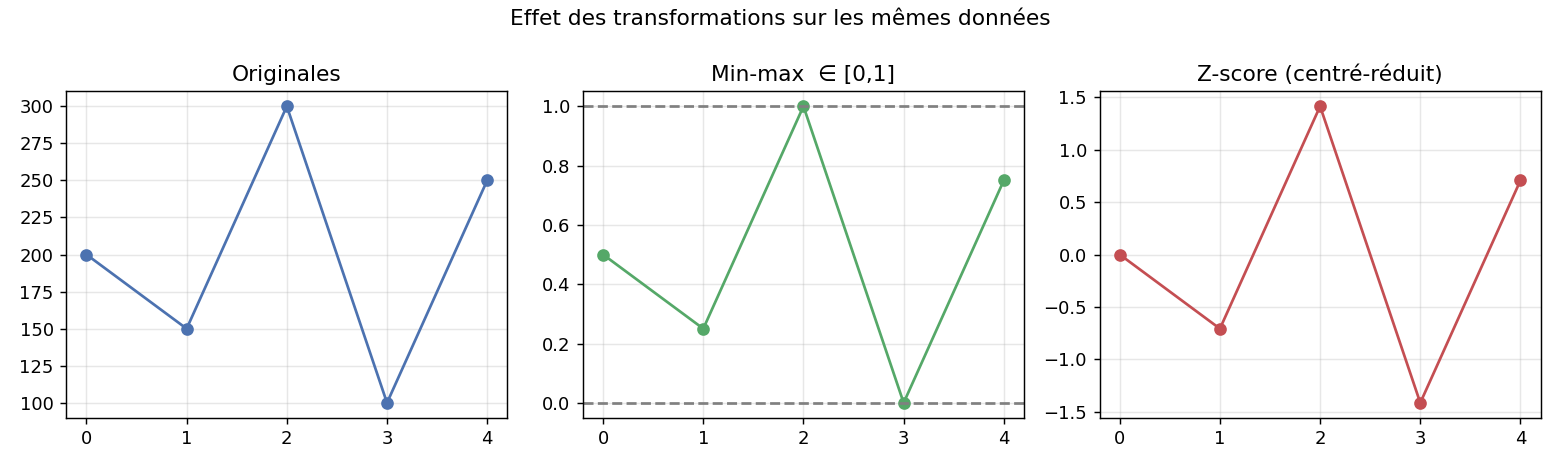
\includegraphics[width=0.95\linewidth]{figures/chap2_transformations.png}
\caption{Mêmes données vues en brut, après min-max (dans $[0,1]$) et après z-score (centré-réduit).}
\end{figure}

\section{Réduction des données}
Obtenir une représentation \textbf{plus petite} mais aux résultats \textbf{quasi identiques} :
agrégation par cubes, \textbf{réduction de dimension} (moins de colonnes/attributs),
réduction de numérosité (moins de lignes), discrétisation.

\section{Exercices résolus}

\subsection{Exercice 1 — repérer les problèmes de qualité}
\begin{center}\small
\begin{tabular}{cccccc}
\toprule
ID & Code postal & Sexe & Revenu & Âge & État civil\\
\midrule
1001 & 10048 & M & 75000 & C & M\\
1002 & J2S7K7 & F & -40000 & 40 & V\\
1003 & 90210 & \cellcolor{rougeclair}(vide) & \cellcolor{rougeclair}10000000 & 45 & C\\
1004 & \cellcolor{rougeclair}6269 & M & 50000 & \cellcolor{rougeclair}0 & C\\
1005 & 55101 & F & \cellcolor{rougeclair}999999 & 30 & D\\
\bottomrule
\end{tabular}
\end{center}

\begin{Calcul}[: problèmes détectés]
\begin{itemize}[leftmargin=1.4em,nosep]
  \item \textbf{Valeur manquante} : sexe absent (ligne 1003).
  \item \textbf{Valeur hors domaine} : revenu $=-40000$ (négatif, impossible).
  \item \textbf{Valeur aberrante} : revenu $=10\,000\,000$ (extrême).
  \item \textbf{Code de manquant déguisé} : revenu $=999999$ et âge $=0$ (faux \og vrais \fg{} chiffres).
  \item \textbf{Incohérence de type/format} : âge $=$ \og C \fg{} (non numérique) ;
        codes postaux mélangeant chiffres US (5 chiffres) et alphanumérique canadien (J2S7K7).
\end{itemize}
\end{Calcul}

\subsection{Exercice 2 — normalisation \& standardisation (dataset \texttt{churn})}
La démarche (que le script automatise) :
\begin{enumerate}[leftmargin=1.6em,nosep]
  \item vérifier les valeurs manquantes (\texttt{df.isna().sum()}) ;
  \item comparer \texttt{area code} et \texttt{state} (incohérences géographiques) ;
  \item transformer \texttt{day minutes} par \textbf{min-max} et vérifier sur une courbe que
        tout est dans $[0,1]$ ;
  \item transformer \texttt{night minutes} par \textbf{z-score} et lire l'intervalle obtenu
        (typiquement $[-3,+3]$).
\end{enumerate}

\section{Script Python commenté}
\lstinputlisting[caption={scripts/chap2\_normalisation.py — min-max, z-score, qualité},
  label=lst:chap2]{../scripts/chap2_normalisation.py}

\begin{Resume}
Prétraiter = nettoyer (manquants, bruit), intégrer (sources, redondance), transformer
(\textbf{min-max} dans $[0,1]$, \textbf{z-score} centré-réduit) et réduire. C'est l'étape la
plus chronophage mais elle conditionne tout le reste — en particulier le K-NN et le k-means
qui dépendent des distances.
\end{Resume}

\chapter{Classification}

\begin{Definition}[Classification]
Raisonnement \textbf{à partir de cas} : on a des enregistrements décrits par des attributs,
dont l'un est la \textbf{classe}. On cherche un \textbf{modèle} qui exprime la classe en
fonction des autres attributs, pour ensuite \textbf{prédire la classe} d'enregistrements
inconnus. C'est de l'apprentissage \textbf{supervisé}.
\end{Definition}

\textbf{Deux étapes :} (1) \emph{construction du modèle} sur l'ensemble d'\textbf{apprentissage}
(\emph{training set}, $\approx 2/3$) ; (2) \emph{utilisation/test} du modèle sur l'ensemble de
\textbf{test} ($\approx 1/3$) pour mesurer la précision. On peut aussi faire de la
\textbf{validation croisée} : découper en $k$ paquets, apprendre sur $k-1$ et tester sur le
dernier, en tournant.

\section{Méthode des $K$ plus proches voisins (K-NN)}

\begin{Definition}[K-NN]
\textbf{Pas d'apprentissage} : le modèle \emph{est} l'échantillon. Pour classer un nouvel
individu $y$ : on calcule sa \textbf{distance} à tous les individus connus, on garde les
\textbf{$K$ plus proches}, et on attribue à $y$ la \textbf{classe majoritaire} parmi ces $K$
voisins. Heuristique : $K = \text{nombre d'attributs} + 1$.
\end{Definition}

\textbf{Vote simple} : chaque voisin compte pour 1. \textbf{Vote pondéré} : chaque voisin a un
poids $\propto 1/\text{distance}$ (plus il est proche, plus il pèse). \textbf{Confiance} $=$
votes gagnants $/$ total des votes.

\textbf{Distances entre numériques} ($x,y\in\R^m$) :
\[ d_{\text{Euclidienne}}=\sqrt{\textstyle\sum_i (x_i-y_i)^2},\quad
   d_{\text{Manhattan}}=\textstyle\sum_i |x_i-y_i|,\quad
   d_{\text{Minkowski}}=\Big(\textstyle\sum_i |x_i-y_i|^q\Big)^{1/q}. \]
($q=1$ : Manhattan ; $q=2$ : Euclidienne.) \textbf{Données nominales} : $d=0$ si égales, $1$
sinon.

\begin{Attention}
K-NN dépend des distances : il faut \textbf{normaliser} les attributs avant, sinon
l'attribut aux grandes valeurs (ex. le salaire) écrase les autres.
\end{Attention}

\subsection{Exercice résolu — classer David ($K=3$, euclidienne)}
\begin{center}\small
\begin{tabular}{lcccc}
\toprule
Client & Âge & Salaire & Nb cartes & Classe (Loyal)\\
\midrule
Jean & 35 & 35000 & 3 & N\\
Rachèle & 22 & 50000 & 2 & O\\
Anne & 63 & 200000 & 1 & N\\
Thomas & 59 & 170000 & 1 & N\\
Nathalie & 25 & 40000 & 4 & O\\
\rowcolor{orangeclair}\textbf{David} & 37 & 50000 & 2 & \textbf{?}\\
\bottomrule
\end{tabular}
\end{center}

\textbf{Démarche, en 3 temps :} (1) on calcule la distance de David à \emph{chacun} des 5
clients connus ; (2) on \emph{trie} ces distances et on garde les $K=3$ plus petites ;
(3) on regarde la classe de ces 3 voisins et on \emph{vote}.

\begin{Calcul}[: distances euclidiennes de David $(37;50000;2)$ à chacun]
On applique $d=\sqrt{(\Delta\text{âge})^2+(\Delta\text{salaire})^2+(\Delta\text{cartes})^2}$.
On écrit \emph{tous} les termes avant de simplifier :
\begin{align*}
d(\text{David},\text{Jean}) &=\sqrt{(37-35)^2+(50000-35000)^2+(2-3)^2}
   =\sqrt{\underbrace{4}_{\text{âge}}+\underbrace{225\,000\,000}_{\text{salaire}}+\underbrace{1}_{\text{cartes}}}\approx \mathbf{15000{,}0}\\
d(\text{David},\text{Rachèle}) &=\sqrt{(37-22)^2+(50000-50000)^2+(2-2)^2}
   =\sqrt{225+0+0}= \mathbf{15{,}0}\\
d(\text{David},\text{Anne}) &=\sqrt{(37-63)^2+(50000-200000)^2+(2-1)^2}
   =\sqrt{676+22\,500\,000\,000+1}\approx \mathbf{150000{,}0}\\
d(\text{David},\text{Thomas}) &=\sqrt{(37-59)^2+(50000-170000)^2+(2-1)^2}
   =\sqrt{484+14\,400\,000\,000+1}\approx \mathbf{120000{,}0}\\
d(\text{David},\text{Nathalie}) &=\sqrt{(37-25)^2+(50000-40000)^2+(2-4)^2}
   =\sqrt{144+100\,000\,000+4}\approx \mathbf{10000{,}0}
\end{align*}
\textbf{Tri croissant} : Rachèle $15$ < Nathalie $10\,000$ < Jean $15\,000$ < Thomas
$120\,000$ < Anne $150\,000$. \\
\textbf{Les $K=3$ plus proches} : Rachèle (\textbf{O}), Nathalie (\textbf{O}), Jean (\textbf{N}).
\end{Calcul}

\begin{Calcul}[: vote simple — détail]
On compte les classes des 3 voisins : \og O \fg{} apparaît 2 fois (Rachèle, Nathalie),
\og N \fg{} 1 fois (Jean).
\[ \text{score}(O)=2,\qquad \text{score}(N)=1 \;\Rightarrow\; \text{classe majoritaire}=\mathbf{O}. \]
\textbf{Confiance} $=\dfrac{\text{voix gagnantes}}{\text{total des voix}}=\dfrac{2}{3}\approx \mathbf{67\,\%}$.
\end{Calcul}

\begin{Calcul}[: vote pondéré — détail]
Chaque voisin pèse $w=1/d$ (proche $\Rightarrow$ gros poids). On additionne les poids
\emph{par classe} :
\[ w_O=\underbrace{\tfrac{1}{15}}_{\text{Rachèle}}+\underbrace{\tfrac{1}{10000}}_{\text{Nathalie}}
   \approx 0{,}06667+0{,}00010=0{,}06677, \qquad
   w_N=\underbrace{\tfrac{1}{15000}}_{\text{Jean}}\approx 0{,}00007. \]
Comme $w_O \gg w_N$, la classe pondérée est \textbf{O}.
Confiance pondérée $=\dfrac{w_O}{w_O+w_N}=\dfrac{0{,}06677}{0{,}06684}\approx \mathbf{99{,}9\,\%}$.
\textbf{Conclusion identique :} David est classé \textbf{O} (Loyal $=$ O).
\end{Calcul}

\begin{Attention}[: le piège des échelles]
Regardez les termes sous la racine : le salaire pèse $\sim 10^8$, l'âge $\sim 10^2$, les
cartes $\sim 1$. \textbf{Le salaire écrase tout} : la distance est, à $0{,}001\,\%$ près, égale
à l'écart de salaire. On ne fait donc, en réalité, du K-NN \emph{que sur le salaire}. C'est
pourquoi le cours recommande de \textbf{normaliser avant un K-NN}.
\end{Attention}

\begin{Calcul}[: la même classification, mais \textbf{normalisée} (min-max)]
On ramène chaque attribut dans $[0,1]$ avec $x^*=\dfrac{x-\min}{\max-\min}$, à partir des
bornes de l'apprentissage : âge $\in[22,63]$ (étendue 41), salaire $\in[35000,200000]$
(étendue 165000), cartes $\in[1,4]$ (étendue 3).\\[3pt]
David $\rightarrow \big(\tfrac{37-22}{41};\tfrac{50000-35000}{165000};\tfrac{2-1}{3}\big)
=(0{,}366;\,0{,}091;\,0{,}333)$. Distances normalisées :
\begin{center}\small
\begin{tabular}{lccccc}
\toprule
& Jean & Rachèle & Anne & Thomas & Nathalie\\
\midrule
distance & \textbf{0,349} (N) & \textbf{0,366} (O) & 1,157 (N) & 0,963 (N) & \textbf{0,731} (O)\\
\bottomrule
\end{tabular}
\end{center}
\textbf{Surprise :} maintenant que les 3 attributs comptent autant, \textbf{Jean (N) devient le
plus proche} ! Mais les 3 plus proches sont Jean (N), Rachèle (O), Nathalie (O) : le vote
donne encore $\mathbf{O}$ (2 contre 1). La normalisation a changé les distances et le
classement, \textbf{pas la décision finale} ici.
\end{Calcul}

\begin{figure}[ht]\centering
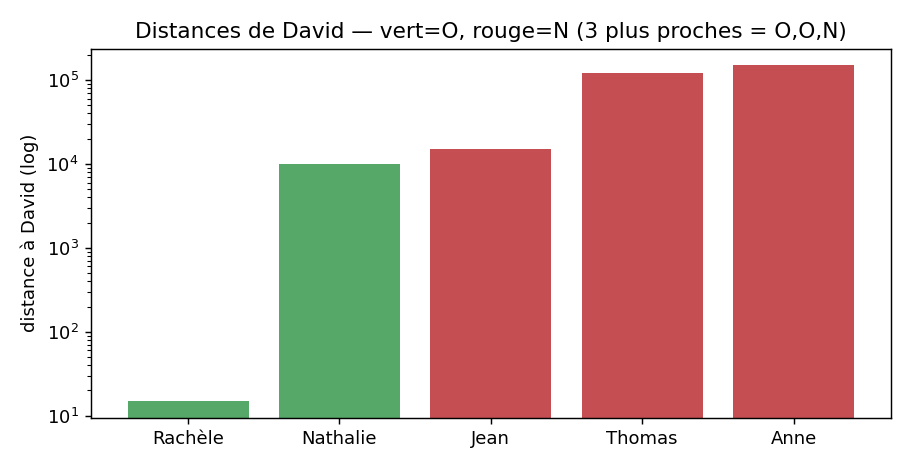
\includegraphics[width=0.7\linewidth]{figures/knn_distances.png}
\caption{Distances brutes de David (échelle log à cause du salaire). Vert $=$ O, rouge $=$ N.
Les 3 plus proches : O, O, N $\Rightarrow$ O.}
\end{figure}

\lstinputlisting[caption={scripts/knn\_david.py},label=lst:knn]{../scripts/knn_david.py}

\section{Arbres de décision}

\begin{Definition}[Arbre de décision]
Représentation graphique d'une procédure de classification. \textbf{Nœud interne} $=$ test
sur un attribut ; \textbf{branche} $=$ résultat du test ; \textbf{feuille} $=$ classe. Chaque
chemin racine$\rightarrow$feuille donne une \textbf{règle SI…ALORS}.
\end{Definition}

\textbf{Construction (récursive)} : (1) toutes les instances à la racine ; (2) choisir le
\textbf{meilleur attribut} de découpage (selon un critère) ; (3) partitionner ; (4) recommencer
sur chaque fils ; (5) arrêter quand le nœud est \textbf{pur} (une seule classe), presque pur,
ou qu'il n'y a plus d'attribut. Critères de choix : \textbf{indice de Gini} (CART),
\textbf{gain d'information} (ID3, C4.5), $\chi^2$ (CHAID).

\subsection{Critère 1 — Indice de Gini}

\begin{Definition}[Gini]
\[ GINI(t)=1-\sum_j \big[p(j|t)\big]^2 \]
$p(j|t)$ $=$ fréquence de la classe $j$ au nœud $t$. \textbf{Gini $=0$} si le nœud est
\textbf{pur} ; plus Gini est \textbf{bas}, plus le nœud est \textbf{pur}.
Pour un découpage en $k$ fils :
\[ GINI_{\text{split}}=\sum_{i=1}^{k}\frac{n_i}{n}\,GINI(i) \quad\text{(à \textbf{minimiser})}. \]
\end{Definition}

\begin{Calcul}[: petits exemples de Gini (sur 6 enregistrements)]
$(C_1{=}0,C_2{=}6)$ : $GINI=1-0^2-1^2=\mathbf{0}$ (pur).\quad
$(C_1{=}1,C_2{=}5)$ : $GINI=1-(\tfrac16)^2-(\tfrac56)^2=\mathbf{0{,}278}$.\quad
$(C_1{=}2,C_2{=}4)$ : $GINI=1-(\tfrac26)^2-(\tfrac46)^2=\mathbf{0{,}444}$.
\end{Calcul}

\paragraph{Exercice résolu (assurance auto).}
\begin{center}\small
\begin{tabular}{ccc}
\toprule
Âge & Type\_voit & Risque\\
\midrule
23 & Familiale & Élevé\\ 17 & Sport & Élevé\\ 43 & Sport & Élevé\\
68 & Familiale & Faible\\ 32 & Camion & Faible\\ 20 & Familiale & Élevé\\
\bottomrule
\end{tabular}
\end{center}

\textbf{Plan :} on évalue chaque attribut comme candidat de découpage de la racine, on garde
celui qui donne le plus petit $GINI_{\text{split}}$, puis on recommence sur chaque fils.

\begin{Calcul}[: étape 0 — impureté de la racine]
La racine contient les 6 enregistrements : 4 \og Élevé \fg{} et 2 \og Faible \fg{}. Les
fréquences sont $p(\text{Élevé})=\tfrac46$ et $p(\text{Faible})=\tfrac26$, donc
\[ GINI(\text{racine})=1-\Big(\tfrac46\Big)^2-\Big(\tfrac26\Big)^2
   =1-\tfrac{16}{36}-\tfrac{4}{36}=1-0{,}444-0{,}111=\mathbf{0{,}444}. \]
\textbf{But :} trouver le découpage qui fait \emph{le plus baisser} cette valeur.
\end{Calcul}

\begin{Calcul}[: candidat A — l'attribut nominal \texttt{Type\_voit}]
Découpage multi-branche, un fils par valeur :
\begin{itemize}[nosep,leftmargin=1.4em]
  \item \textbf{Familiale} $=\{$Élevé (23), Faible (68), Élevé (20)$\}$ : 2 Élevé, 1 Faible,
        donc $GINI=1-(\tfrac23)^2-(\tfrac13)^2=1-0{,}444-0{,}111=0{,}444$ ;
  \item \textbf{Sport} $=\{$Élevé (17), Élevé (43)$\}$ : \emph{pur} $\Rightarrow GINI=0$ ;
  \item \textbf{Camion} $=\{$Faible (32)$\}$ : \emph{pur} $\Rightarrow GINI=0$.
\end{itemize}
Moyenne pondérée par la taille des fils ($3,2,1$ sur $6$) :
\[ GINI_{\text{split}}=\tfrac36(0{,}444)+\tfrac26(0)+\tfrac16(0)=\mathbf{0{,}222}. \]
\end{Calcul}

\begin{Calcul}[: candidat B — l'attribut continu \texttt{Âge} (on teste \emph{tous} les seuils)]
On trie les âges et leur classe : $17_{\text{É}}, 20_{\text{É}}, 23_{\text{É}}, 32_{\text{F}},
43_{\text{É}}, 68_{\text{F}}$. Un seuil candidat est le \emph{milieu} de deux âges consécutifs.
\begin{center}\small
\renewcommand{\arraystretch}{1.3}
\begin{tabular}{c l l c}
\toprule
Seuil & Gauche (Âge $<$ seuil) & Droite (Âge $\geq$ seuil) & $GINI_{\text{split}}$\\
\midrule
18,5 & $\{17\}$ : É — pur, $0$ & $\{20,23,32,43,68\}$ : 3É,2F, $0{,}48$ &
  $\tfrac16(0)+\tfrac56(0{,}48)=0{,}400$\\
21,5 & $\{17,20\}$ : pur, $0$ & $\{23,32,43,68\}$ : 2É,2F, $0{,}50$ &
  $\tfrac26(0)+\tfrac46(0{,}50)=0{,}333$\\
\rowcolor{vertclair}\textbf{27,5} & $\{17,20,23\}$ : pur, $0$ & $\{32,43,68\}$ : 1É,2F, $0{,}444$ &
  $\tfrac36(0)+\tfrac36(0{,}444)=\mathbf{0{,}222}$\\
37,5 & $\{17,20,23,32\}$ : 3É,1F, $0{,}375$ & $\{43,68\}$ : 1É,1F, $0{,}50$ &
  $\tfrac46(0{,}375)+\tfrac26(0{,}50)=0{,}417$\\
55,5 & $\{17,20,23,32,43\}$ : 4É,1F, $0{,}32$ & $\{68\}$ : pur, $0$ &
  $\tfrac56(0{,}32)+\tfrac16(0)=0{,}267$\\
\bottomrule
\end{tabular}
\end{center}
Le \textbf{meilleur seuil} est $\text{Âge}<27{,}5$ avec $GINI_{\text{split}}=\mathbf{0{,}222}$
(détail d'un $GINI$ de fils : pour la droite $\{32,43,68\}$, 1 Élevé et 2 Faible donnent
$1-(\tfrac13)^2-(\tfrac23)^2=0{,}444$).
\end{Calcul}

\begin{Astuce}[: pourquoi Âge $<27{,}5$ et pas \texttt{Type\_voit} ?]
Les deux donnent $GINI_{\text{split}}=0{,}222$ : \textbf{égalité parfaite}. En cas d'égalité,
CART/scikit-learn tranche selon l'ordre interne des variables et choisit ici
\textbf{Âge $<27{,}5$}. On suit ce choix (l'autre arbre, démarrant par \texttt{Type\_voit},
serait tout aussi correct).
\end{Astuce}

\begin{Calcul}[: 2\textsuperscript{e} niveau — le fils \og Âge $\geq 27{,}5$ \fg{}]
Le fils gauche (\og Âge $<27{,}5$ \fg{}) est \emph{pur} (tous Élevé) : c'est une feuille,
on s'arrête. Le fils droit contient $\{32_{\text{Camion,F}}, 43_{\text{Sport,É}},
68_{\text{Familiale,F}}\}$, soit 1 Élevé et 2 Faible : $GINI=0{,}444$, il faut le re-découper.
\begin{itemize}[nosep,leftmargin=1.4em]
  \item \textbf{Par \texttt{Type\_voit}} : Sport$\to\{$É$\}$ pur, Familiale$\to\{$F$\}$ pur,
        Camion$\to\{$F$\}$ pur. $GINI_{\text{split}}=\mathbf{0}$ — \textbf{séparation parfaite}.
  \item \textbf{Par \texttt{Âge}} (seuils 37,5 et 55,5) : on retombe à chaque fois sur
        $GINI_{\text{split}}=\tfrac13(0)+\tfrac23(0{,}5)=0{,}333$.
\end{itemize}
$0 < 0{,}333$ : on choisit donc \texttt{Type\_voit}, qui classe parfaitement les 3 derniers cas.
\end{Calcul}

\begin{Exemple}[arbre Gini final]
{\ttfamily\setlength{\parindent}{0pt}
Âge < 27,5 ?\\
\quad |-- OUI ~~> \textbf{Élevé}\\
\quad |-- NON ~~> Type\_voit ?\\
\quad\qquad\quad |-- Sport ~~> \textbf{Élevé}\\
\quad\qquad\quad |-- Familiale ~~> \textbf{Faible}\\
\quad\qquad\quad |-- Camion ~~> \textbf{Faible}
}
\end{Exemple}

\begin{figure}[ht]\centering
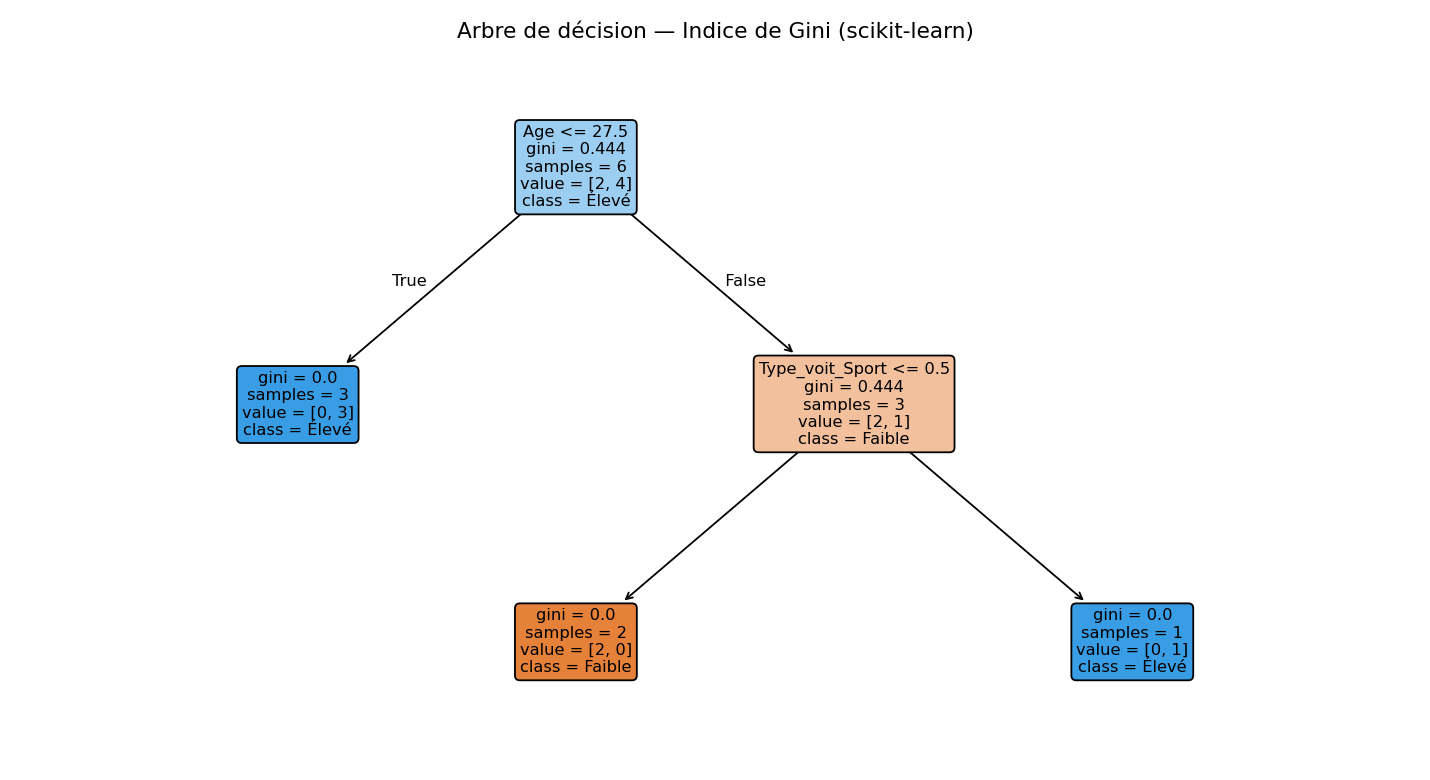
\includegraphics[width=0.85\linewidth]{figures/gini_arbre.png}
\caption{Arbre de décision Gini reconstruit par scikit-learn (\texttt{Type\_voit} encodé en one-hot).}
\end{figure}

\lstinputlisting[caption={scripts/gini\_arbre.py},label=lst:gini]{../scripts/gini_arbre.py}

\subsection{Critère 2 — Gain d'information (entropie)}

\begin{Definition}[Entropie et gain]
\[ Entropie(t)=-\sum_j p(j|t)\log_2 p(j|t),\qquad
   GAIN_{\text{split}}=Entropie(p)-\sum_{i=1}^{k}\frac{n_i}{n}Entropie(i). \]
Entropie $=0$ si pur, maximale ($\log_2 n_c$) si classes équilibrées. On choisit l'attribut
qui \textbf{maximise le gain} (la plus grande réduction d'entropie). \textbf{C4.5} corrige en
divisant par le \emph{SplitINFO} (\emph{gain ratio}) pour pénaliser les attributs à trop de
valeurs.
\end{Definition}

\begin{Calcul}[: comprendre l'entropie sur 3 cas (6 enregistrements)]
On note $\log_2 x=\dfrac{\ln x}{\ln 2}$. Plus le mélange est équilibré, plus l'entropie est grande.
\begin{itemize}[nosep,leftmargin=1.4em]
  \item $(C_1{=}0,C_2{=}6)$ : tout dans une classe.
        $-\tfrac06\log_2\tfrac06-\tfrac66\log_2\tfrac66=-0-1\cdot\log_2 1=-0-0=\mathbf{0}$
        (nœud \emph{pur}).
  \item $(C_1{=}1,C_2{=}5)$ : $-\tfrac16\log_2\tfrac16-\tfrac56\log_2\tfrac56
        =-\tfrac16(-2{,}585)-\tfrac56(-0{,}263)=0{,}431+0{,}219=\mathbf{0{,}650}$.
  \item $(C_1{=}2,C_2{=}4)$ : $-\tfrac26\log_2\tfrac26-\tfrac46\log_2\tfrac46
        =-\tfrac13(-1{,}585)-\tfrac23(-0{,}585)=0{,}528+0{,}390=\mathbf{0{,}918}$.
\end{itemize}
\end{Calcul}

\paragraph{Exercice résolu (achat d'ordinateur, 14 individus).} C'est l'exemple du TP.
Classe \texttt{Achète\_ordinateur} : \textbf{9 \og oui \fg{}} et \textbf{5 \og non \fg{}}.

\begin{Calcul}[: étape 0 — entropie de la racine]
\[ Entropie(S)=-\tfrac{9}{14}\log_2\tfrac{9}{14}-\tfrac{5}{14}\log_2\tfrac{5}{14}
   =-0{,}643\cdot(-0{,}637)-0{,}357\cdot(-1{,}485)=0{,}410+0{,}530=\mathbf{0{,}940}. \]
\end{Calcul}

\begin{Calcul}[: gain de l'attribut \texttt{Âge}]
\texttt{Âge} a 3 valeurs. On compte les classes dans chaque groupe, puis son entropie :
\begin{itemize}[nosep,leftmargin=1.4em]
  \item $\le 30$ : 5 individus, \textbf{2 oui / 3 non} $\Rightarrow
        -\tfrac25\log_2\tfrac25-\tfrac35\log_2\tfrac35=0{,}529+0{,}442=0{,}971$ ;
  \item $31..40$ : 4 individus, \textbf{4 oui / 0 non} $\Rightarrow$ pur, entropie $=0$ ;
  \item $>40$ : 5 individus, \textbf{3 oui / 2 non} $\Rightarrow 0{,}971$ (symétrique du premier).
\end{itemize}
Entropie restante (pondérée par $5,4,5$ sur $14$) :
\[ E_{\text{reste}}=\tfrac{5}{14}(0{,}971)+\tfrac{4}{14}(0)+\tfrac{5}{14}(0{,}971)=0{,}694
   \;\Rightarrow\; \boxed{GAIN(\text{Âge})=0{,}940-0{,}694=0{,}247}. \]
\end{Calcul}

\begin{Calcul}[: gain des trois autres attributs]
\textbf{\texttt{Revenue}} (élevé : 2o/2n $\to1{,}0$ ; moyen : 4o/2n $\to0{,}918$ ; bas : 3o/1n $\to0{,}811$) :
\[ E_{\text{reste}}=\tfrac{4}{14}(1)+\tfrac{6}{14}(0{,}918)+\tfrac{4}{14}(0{,}811)=0{,}911
   \;\Rightarrow\; GAIN=\mathbf{0{,}029}. \]
\textbf{\texttt{Étudiant}} (oui : 6o/1n $\to0{,}592$ ; non : 3o/4n $\to0{,}985$) :
\[ E_{\text{reste}}=\tfrac{7}{14}(0{,}592)+\tfrac{7}{14}(0{,}985)=0{,}789
   \;\Rightarrow\; GAIN=\mathbf{0{,}151}. \]
\textbf{\texttt{État\_civil}} (célibataire : 6o/2n $\to0{,}811$ ; marié : 3o/3n $\to1{,}0$) :
\[ E_{\text{reste}}=\tfrac{8}{14}(0{,}811)+\tfrac{6}{14}(1)=0{,}892
   \;\Rightarrow\; GAIN=\mathbf{0{,}048}. \]
\end{Calcul}

\begin{Astuce}[: choix de la racine]
\begin{center}\small
\begin{tabular}{lcccc}
\toprule
Attribut & \textbf{Âge} & Étudiant & État\_civil & Revenue\\
\midrule
Gain & \cellcolor{vertclair}\textbf{0,247} & 0,151 & 0,048 & 0,029\\
\bottomrule
\end{tabular}
\end{center}
\texttt{Âge} a le \textbf{plus grand gain} (réduit le plus l'entropie) : c'est la \textbf{racine}.
\end{Astuce}

\begin{Calcul}[: 2\textsuperscript{e} niveau — re-découper chaque fils de l'âge]
\textbf{Âge $=31..40$} : déjà pur (4 oui) $\Rightarrow$ \textbf{feuille \og oui \fg{}}, on s'arrête.\\[3pt]
\textbf{Âge $\le 30$} (2 oui, 3 non, entropie $0{,}971$). On recalcule le gain des attributs
\emph{restants} dans ce sous-ensemble de 5 individus :
\begin{itemize}[nosep,leftmargin=1.4em]
  \item \texttt{Étudiant} : oui$\to\{$oui,oui$\}$ (pur), non$\to\{$non,non,non$\}$ (pur)
        $\Rightarrow E_{\text{reste}}=0$, \textbf{gain $=0{,}971$ (maximal)} ;
  \item \texttt{Revenue} : gain $=0{,}571$ ; \quad \texttt{État\_civil} : gain $=0{,}020$.
\end{itemize}
$\Rightarrow$ on découpe sur \textbf{\texttt{Étudiant}} (sépare parfaitement).\\[3pt]
\textbf{Âge $>40$} (3 oui, 2 non, entropie $0{,}971$) :
\begin{itemize}[nosep,leftmargin=1.4em]
  \item \texttt{État\_civil} : célibataire$\to\{$3 oui$\}$ (pur), marié$\to\{$2 non$\}$ (pur)
        $\Rightarrow$ \textbf{gain $=0{,}971$ (maximal)} ;
  \item \texttt{Étudiant} : gain $=0{,}020$ ; \quad \texttt{Revenue} : gain $=0{,}020$.
\end{itemize}
$\Rightarrow$ on découpe sur \textbf{\texttt{État\_civil}} (sépare parfaitement).
\end{Calcul}

\begin{Exemple}[arbre gain d'information final]
{\ttfamily\setlength{\parindent}{0pt}
Âge ?\\
\quad |-- (<= 30) ~~> Étudiant ?~~ oui ~~> \textbf{oui} ~/~ non ~~> \textbf{non}\\
\quad |-- (31..40) ~~> \textbf{oui}\\
\quad |-- (> 40) ~~> État\_civil ?~~ célibataire ~~> \textbf{oui} ~/~ marié ~~> \textbf{non}
}
\end{Exemple}

\begin{figure}[ht]\centering
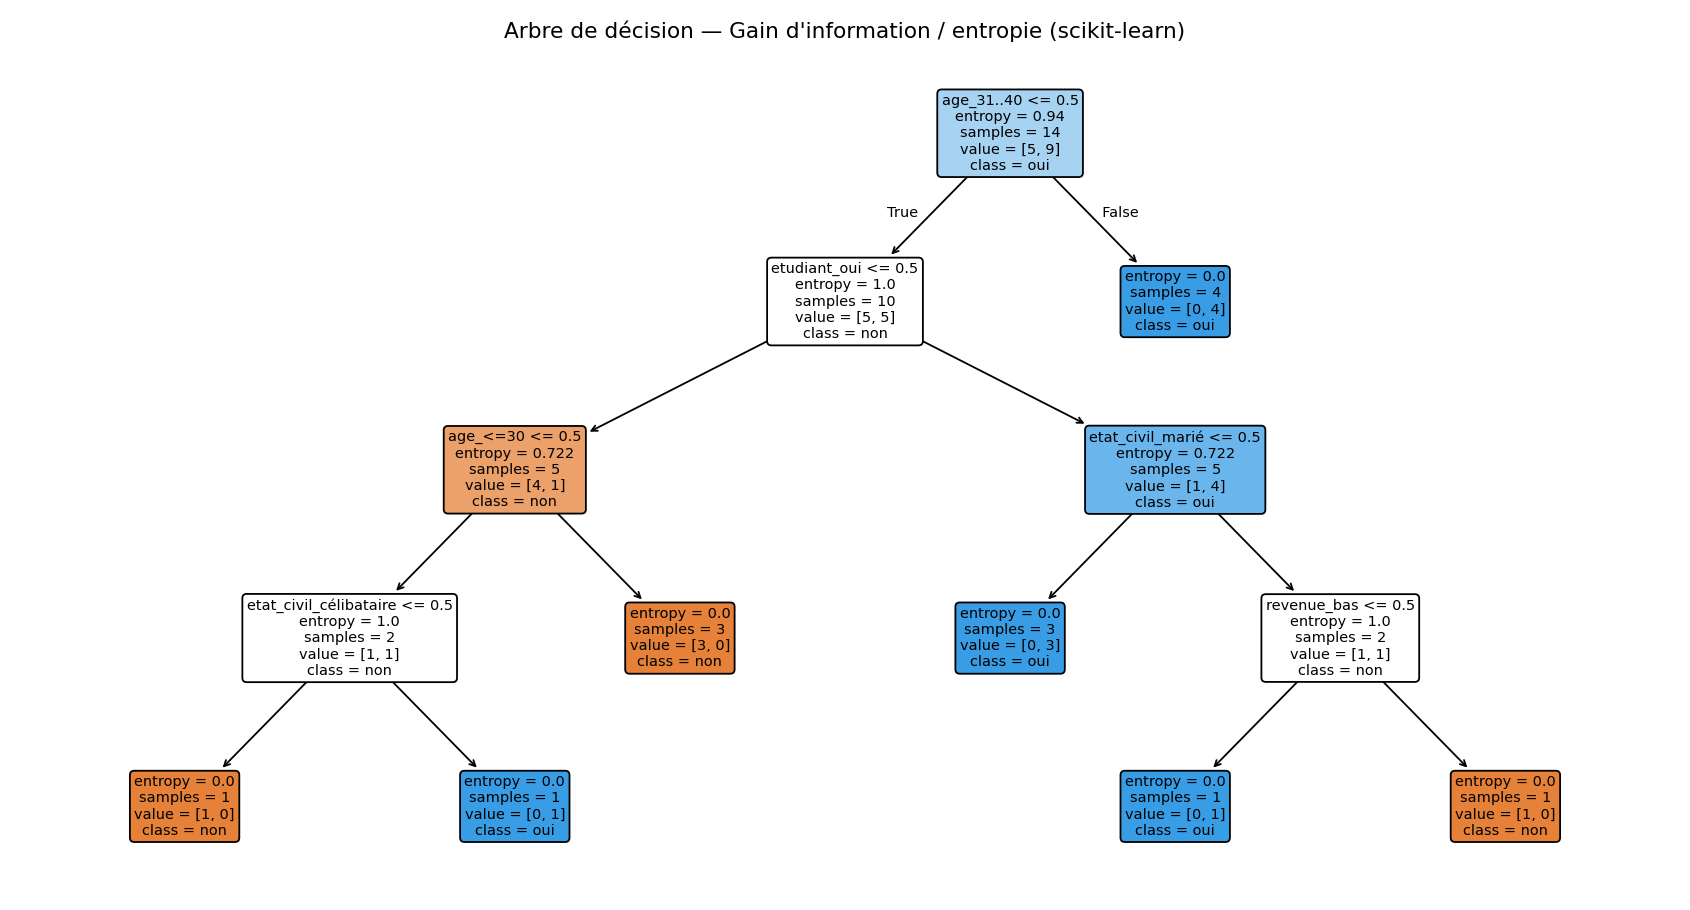
\includegraphics[width=\linewidth]{figures/gain_information_arbre.png}
\caption{Arbre par gain d'information (entropie) reconstruit par scikit-learn.}
\end{figure}

\lstinputlisting[caption={scripts/gain\_information.py},label=lst:gain]{../scripts/gain_information.py}

\section{Mesures de performance}

À partir de la \textbf{matrice de confusion} (cas binaire) :
\begin{center}
\begin{tabular}{l|cc}
& prédit positif & prédit négatif\\\hline
réel positif & TP (vrais positifs) & FN (faux négatifs)\\
réel négatif & FP (faux positifs) & TN (vrais négatifs)\\
\end{tabular}
\end{center}

\[ \text{Exactitude}=\frac{TP+TN}{TP+TN+FP+FN},\quad
   \text{Précision}=\frac{TP}{TP+FP},\quad
   \text{Rappel}=\frac{TP}{TP+FN} \]
\[ \text{Spécificité}=\frac{TN}{TN+FP},\qquad
   F_1=\frac{2\cdot \text{Précision}\cdot \text{Rappel}}{\text{Précision}+\text{Rappel}}. \]

\begin{Calcul}[: exemple TP=40, FN=10, FP=5, TN=45]
Exactitude $=\tfrac{40+45}{100}=0{,}85$ ; Précision $=\tfrac{40}{45}=0{,}889$ ;
Rappel $=\tfrac{40}{50}=0{,}80$ ; Spécificité $=\tfrac{45}{50}=0{,}90$ ;
$F_1=\tfrac{2\cdot0{,}889\cdot0{,}80}{0{,}889+0{,}80}=0{,}842$.
\end{Calcul}

\textbf{Multi-classes} : matrice $m\times m$, bonnes affectations $S=\sum_i n_{ii}$ (diagonale),
taux d'erreur $E=1-\frac{\sum_i n_{ii}}{\sum_{i,j} n_{ij}}$.

\begin{figure}[ht]\centering
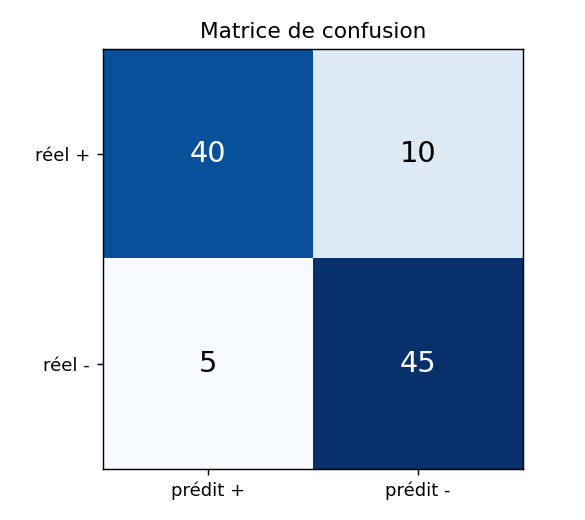
\includegraphics[width=0.4\linewidth]{figures/matrice_confusion.png}
\caption{Matrice de confusion de l'exemple.}
\end{figure}

\lstinputlisting[caption={scripts/performance\_classification.py},label=lst:perf]{../scripts/performance_classification.py}

\begin{Resume}
\textbf{K-NN} : pas d'apprentissage, on vote parmi les $K$ voisins les plus proches
(normaliser avant !). \textbf{Arbres} : on découpe récursivement selon le meilleur attribut —
\textbf{Gini} (à minimiser, CART) ou \textbf{gain d'information} (à maximiser, ID3/C4.5).
\textbf{Performance} : matrice de confusion $\rightarrow$ exactitude, précision, rappel, $F_1$.
\end{Resume}

\chapter{Segmentation (Clustering)}

\begin{Definition}[Clustering]
Organiser les données en \textbf{groupes (clusters)} de sorte que les données
\textbf{similaires} soient ensemble. C'est de l'apprentissage \textbf{non supervisé} :
\textbf{les classes sont inconnues}, on les découvre.
\end{Definition}

\begin{Astuce}[: ce qu'est un \og bon \fg{} clustering]
\textbf{Forte similarité \emph{intra}-classe} (les points d'un même groupe se ressemblent)
\textbf{et faible similarité \emph{inter}-classes} (les groupes sont bien séparés).
\end{Astuce}

\section{Mesurer la qualité d'un cluster}
Chaque cluster $C_k$ ($N_k$ points) est caractérisé par :
\[ \text{centre de gravité } \mu_k=\frac{1}{N_k}\sum_{x_i\in C_k} x_i, \qquad
   \text{inertie } J_k=\sum_{x_i\in C_k} d^2(x_i,\mu_k). \]
\textbf{Inertie intra} (faible $=$ points concentrés autour du centre) ; \textbf{inertie inter}
(grande $=$ centres éloignés, clusters bien séparés). \textbf{Objectif :} minimiser l'intra et
maximiser l'inter.

\section{Clustering hiérarchique}
On construit un \textbf{dendrogramme} (arbre binaire de groupes). On le \textbf{coupe}
horizontalement pour obtenir le nombre de groupes voulu.
\begin{itemize}[leftmargin=1.4em,nosep]
  \item \textbf{Ascendant (agglomératif)} — le plus courant : on part de $n$ singletons et on
        \textbf{fusionne} les groupes les plus proches jusqu'à un seul groupe.
  \item \textbf{Descendant (divisif)} : on part d'un groupe et on le divise.
\end{itemize}
\textbf{Distance entre groupes} : \textbf{lien simple} (min des distances), \textbf{lien complet}
(max), \textbf{lien moyen} (moyenne).

\subsection{Exercice résolu — lien simple}
Matrice de distance :
\begin{center}\small
\begin{tabular}{c|cccc}
 & B & C & D & E\\\hline
A & 1 & 3 & 2 & 4\\
B &   & 3 & 2 & 3\\
C &   &   & 1 & 3\\
D &   &   &   & 5\\
\end{tabular}
\end{center}

\begin{Calcul}[: fusions successives (lien simple = min)]
\textbf{Étape 1} : plus petite distance $=1$ pour $(A,B)$ et $(C,D)$. On fusionne
$\mathbf{\{A,B\}}$ (distance 1). Mise à jour (min) :
$d(\{A,B\},C)=\min(3,3)=3$, $d(\{A,B\},D)=\min(2,2)=2$, $d(\{A,B\},E)=\min(4,3)=3$.\\[3pt]
\textbf{Étape 2} : plus petite $=d(C,D)=1$ $\rightarrow$ fusion $\mathbf{\{C,D\}}$. Mise à jour :
$d(\{A,B\},\{C,D\})=\min(3,2)=2$, $d(\{C,D\},E)=\min(3,5)=3$.\\[3pt]
\textbf{Étape 3} : plus petite $=d(\{A,B\},\{C,D\})=2$ $\rightarrow$ fusion
$\mathbf{\{A,B,C,D\}}$. Reste $d(\{A,B,C,D\},E)=\min(3,3)=3$.\\[3pt]
\textbf{Étape 4} : fusion finale avec $E$ à la hauteur \textbf{3}.
\end{Calcul}

\begin{Exemple}[dendrogramme]
Hauteurs de fusion : $\{A,B\}$ et $\{C,D\}$ à $\mathbf{1}$, puis $\{AB,CD\}$ à $\mathbf{2}$,
puis $\{ABCD,E\}$ à $\mathbf{3}$. En coupant à hauteur $2{,}5$ on obtient \textbf{2 groupes} :
$\{A,B,C,D\}$ et $\{E\}$.
\end{Exemple}

\begin{Astuce}[: et avec un autre lien ? (comparaison sur la même matrice)]
Le \emph{lien} change la façon de mesurer la distance entre groupes, donc les hauteurs de
fusion. Sur la même matrice :
\begin{center}\small
\renewcommand{\arraystretch}{1.25}
\begin{tabular}{l l}
\toprule
Lien & Fusions (groupe @ hauteur)\\
\midrule
\textbf{Simple} (min) & $\{AB\}@1,\ \{CD\}@1,\ \{ABCD\}@\mathbf{2},\ \{ABCDE\}@\mathbf{3}$\\
\textbf{Complet} (max) & $\{AB\}@1,\ \{CD\}@1,\ \{ABCD\}@\mathbf{3},\ \{ABCDE\}@\mathbf{5}$\\
\bottomrule
\end{tabular}
\end{center}
Détail du \emph{lien complet} (on prend le \emph{max}) : après $\{A,B\}$ et $\{C,D\}$,
$d(\{A,B\},\{C,D\})=\max(3,2,3,2)=3$ (au lieu de $2$), et la dernière fusion avec $E$ se fait
à $\max(4,3,3,5)=5$ (au lieu de $3$). Le lien complet donne des clusters plus \og compacts \fg{},
le lien simple peut produire des \og chaînes \fg{} allongées.
\end{Astuce}

\begin{figure}[ht]\centering
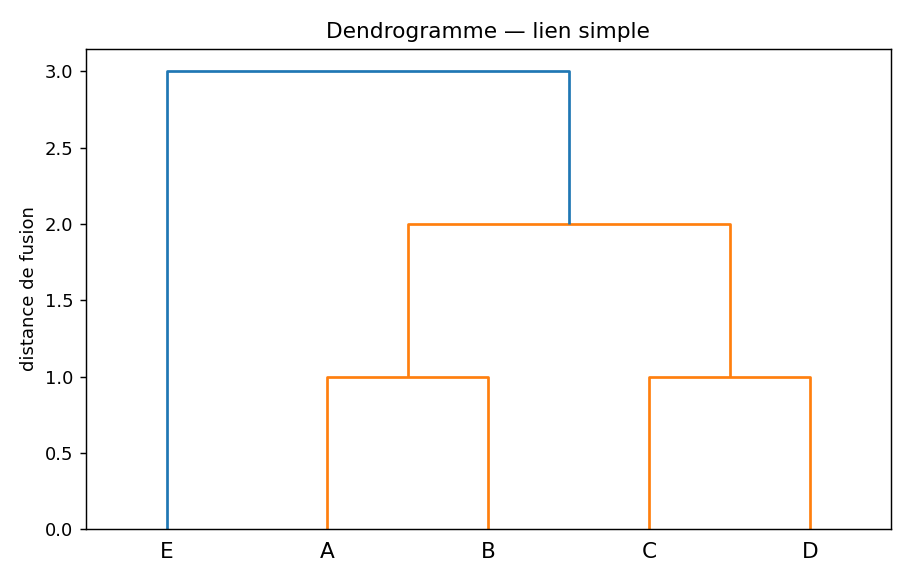
\includegraphics[width=0.55\linewidth]{figures/hierarchique_dendrogramme.png}
\caption{Dendrogramme (lien simple) obtenu avec SciPy — cohérent avec le calcul à la main.}
\end{figure}

\lstinputlisting[caption={scripts/hierarchique\_lien\_simple.py},label=lst:hier]{../scripts/hierarchique_lien_simple.py}

\section{Clustering par partitionnement — K-means}

\begin{Definition}[K-means]
On fixe $K$ à l'avance. On alterne deux étapes jusqu'à convergence :
\textbf{(1) Affectation} — chaque point va au centre $\mu_\ell$ le plus proche ;
\textbf{(2) Mise à jour} — chaque centre devient la \emph{moyenne} de son cluster.
Critère d'arrêt : les centres ne bougent plus,
$\sum_i \|\mu_i^{t}-\mu_i^{t-1}\|^2 \le \epsilon$.
\end{Definition}

\subsection{Exercice résolu — $C=\{2,3,4,10,11,12,20,25,30\}$, $K=2$, $\mu_1=2,\mu_2=4$}

À chaque itération : pour chaque point on compare $|x-\mu_1|$ et $|x-\mu_2|$, on l'affecte au
plus petit ; puis on recalcule chaque centre comme \emph{moyenne} de son groupe.

\begin{Calcul}[: itération 1 en entier ($\mu_1{=}2,\mu_2{=}4$)]
\begin{center}\small
\begin{tabular}{ccccc}
\toprule
$x$ & $|x-2|$ & $|x-4|$ & le plus proche & groupe\\
\midrule
2 & 0 & 2 & $\mu_1$ & $C_1$\\
3 & 1 & 1 & égalité $\to\mu_1$ & $C_1$\\
4 & 2 & 0 & $\mu_2$ & $C_2$\\
10,11,12,20,25,30 & grand & moins grand & $\mu_2$ & $C_2$\\
\bottomrule
\end{tabular}
\end{center}
$C_1=\{2,3\}\to\mu_1=\tfrac{2+3}{2}=2{,}5$ ;\quad
$C_2=\{4,10,11,12,20,25,30\}\to\mu_2=\tfrac{112}{7}=16$.
\end{Calcul}

\begin{Calcul}[: itérations 2 à 5 (résumé des recalculs)]
\textbf{It.\ 2} ($2{,}5;16$) : $C_1=\{2,3,4\}\to\mu_1=3$ ; $C_2=\{10,\dots,30\}\to\mu_2=18$.\\
\textbf{It.\ 3} ($3;18$) : $10$ bascule en $C_1$ car $|10-3|=7<|10-18|=8$.
$C_1=\{2,3,4,10\}\to\mu_1=4{,}75$ ; $C_2=\{11,12,20,25,30\}\to\mu_2=19{,}6$.\\
\textbf{It.\ 4} ($4{,}75;19{,}6$) : $11$ et $12$ basculent en $C_1$ ($|12-4{,}75|=7{,}25<|12-19{,}6|=7{,}6$).
$C_1=\{2,3,4,10,11,12\}\to\mu_1=7$ ; $C_2=\{20,25,30\}\to\mu_2=25$.\\
\textbf{It.\ 5} ($7;25$) : aucune réaffectation, mêmes moyennes $\Rightarrow$
\textbf{convergence} ($\sum_i\|\mu_i^{t}-\mu_i^{t-1}\|^2=0\le\epsilon$).
\end{Calcul}

\begin{Exemple}[résultat]
$\boxed{C_1=\{2,3,4,10,11,12\}\ (\text{centre }7) \qquad C_2=\{20,25,30\}\ (\text{centre }25)}$
\end{Exemple}

\begin{Calcul}[: qualité finale — l'inertie (intra-cluster)]
$J_k=\sum_{x\in C_k}(x-\mu_k)^2$ mesure la dispersion d'un cluster autour de son centre.
\begin{align*}
J_1 &=(2{-}7)^2+(3{-}7)^2+(4{-}7)^2+(10{-}7)^2+(11{-}7)^2+(12{-}7)^2=25{+}16{+}9{+}9{+}16{+}25=100\\
J_2 &=(20{-}25)^2+(25{-}25)^2+(30{-}25)^2=25{+}0{+}25=50
\end{align*}
\textbf{Inertie totale} $J=J_1+J_2=\mathbf{150}$. C'est exactement le \emph{within-cluster
sum of squares} affiché par scikit-learn (\texttt{inertia\_}) et par WEKA. Plus elle est
faible, plus les clusters sont \og serrés \fg{}.
\end{Calcul}

\begin{figure}[ht]\centering
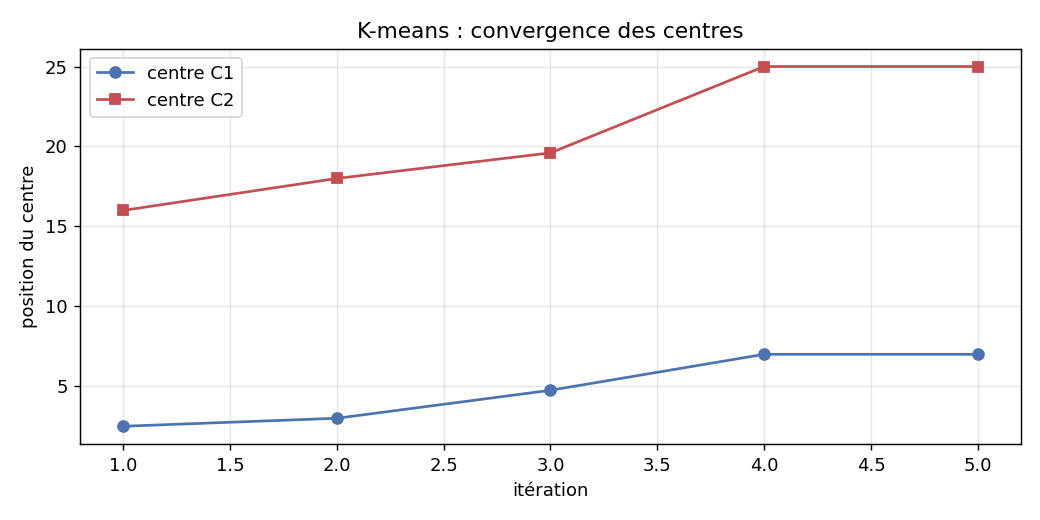
\includegraphics[width=0.49\linewidth]{figures/kmeans_convergence.png}
\hfill
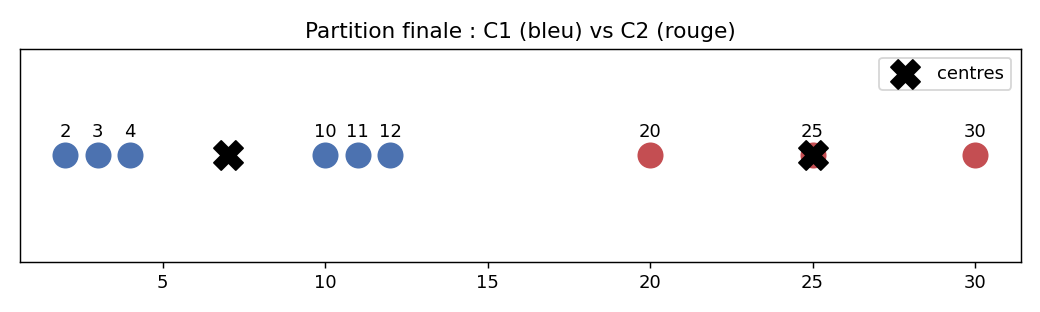
\includegraphics[width=0.49\linewidth]{figures/kmeans_partition.png}
\caption{À gauche : déplacement des centres au fil des itérations. À droite : partition finale.}
\end{figure}

\begin{Attention}
K-means dépend de l'\textbf{initialisation} des centres et exige des \textbf{distances}
(donc \textbf{normaliser} les attributs). Il faut aussi \textbf{choisir $K$} (méthode du coude,
silhouette\dots).
\end{Attention}

\lstinputlisting[caption={scripts/kmeans\_1d.py},label=lst:kmeans]{../scripts/kmeans_1d.py}

\begin{Resume}
\textbf{Hiérarchique} : fusions successives (lien simple/complet/moyen) $\rightarrow$
dendrogramme que l'on coupe. \textbf{K-means} : $K$ fixé, on alterne
affectation $\leftrightarrow$ recalcul des moyennes jusqu'à stabilité. Les deux cherchent
\textbf{forte cohésion interne} et \textbf{forte séparation} entre groupes.
\end{Resume}

\chapter{TP \og CLASSIFICATION \fg{} — corrigé complet}

Ce TP (document scanné) demande de \textbf{dessiner deux arbres de décision} et de
\textbf{vérifier avec WEKA et PYTHON}. Les deux exercices reprennent exactement les jeux de
données traités au chapitre~4 ; on en redonne ici la résolution condensée et la procédure de
vérification.

\section{Exercice 1 — Indice de Gini}
\begin{center}\small
\begin{tabular}{cccc}
\toprule
ID & Âge & Type\_voit & Risque\\
\midrule
0 & 23 & Familiale & Élevé\\ 1 & 17 & Sport & Élevé\\ 2 & 43 & Sport & Élevé\\
3 & 68 & Familiale & Faible\\ 4 & 32 & Camion & Faible\\ 5 & 20 & Familiale & Élevé\\
\bottomrule
\end{tabular}
\end{center}

\textbf{Résolution} (détaillée au \S4.2.1) : $GINI(\text{racine})=0{,}444$. Les deux meilleurs
premiers découpages (Type\_voit et Âge $<27{,}5$) sont à égalité ($GINI_{\text{split}}=0{,}222$) ;
scikit-learn retient \textbf{Âge $<27{,}5$}, puis \textbf{Type\_voit} sépare parfaitement.

\begin{Exemple}[arbre attendu]
\texttt{Âge < 27,5 ?} $\rightarrow$ OUI : \textbf{Élevé} ; NON : \texttt{Type\_voit} $\rightarrow$ Sport=\textbf{Élevé},
Familiale=\textbf{Faible}, Camion=\textbf{Faible}. \\
\textbf{Script :} \texttt{uv run python scripts/gini\_arbre.py} (figure \texttt{gini\_arbre.png}).
\end{Exemple}

\section{Exercice 2 — Gain d'information}
Jeu \og achat d'ordinateur \fg{} (14 lignes, \S4.2.2) : $Entropie(S)=0{,}940$. Gains :
$\text{Âge}=0{,}246$ (max), Étudiant $=0{,}151$, État\_civil $=0{,}048$, Revenue $=0{,}029$.

\begin{Exemple}[arbre attendu]
\texttt{Âge ?} $\rightarrow$ $\le30$ : \texttt{Étudiant} (oui=oui, non=non) ; $31..40$ : \textbf{oui} ;
$>40$ : \texttt{État\_civil} (célibataire=oui, marié=non).\\
\textbf{Script :} \texttt{uv run python scripts/gain\_information.py} (figure
\texttt{gain\_information\_arbre.png}).
\end{Exemple}

\section{Vérification sous WEKA}
\begin{enumerate}[leftmargin=1.6em,nosep]
  \item Enregistrer le tableau au format \texttt{.arff} ou \texttt{.csv}.
  \item \emph{Explorer} $\rightarrow$ onglet \emph{Classify}.
  \item Choisir \texttt{trees > J48} (implémentation de C4.5, $\approx$ gain d'information) ou
        \texttt{trees > SimpleCart} (indice de Gini).
  \item \emph{Test options} : \og Use training set \fg{} (jeux minuscules) puis lancer.
  \item Lire l'arbre dans la sortie texte et le comparer à celui de Python — \textbf{ils
        coïncident} (même attribut racine, mêmes feuilles).
\end{enumerate}

\begin{Astuce}
WEKA J48 utilise le \emph{gain ratio} (C4.5) : sur ces petits jeux, le résultat est identique
à l'arbre par gain d'information ci-dessus. Pour Gini, utiliser SimpleCart/CART.
\end{Astuce}

\begin{Resume}
Les deux arbres du TP sont exactement ceux du chapitre~4. Python (scikit-learn) et WEKA
(J48 / SimpleCart) reconstruisent les mêmes structures, ce qui valide la résolution manuelle.
\end{Resume}

\chapter{Le projet de Data Mining — application Streamlit}

\section{Le sujet}
\begin{Definition}[Cahier des charges]
Concevoir une \textbf{application graphique} (Java ou Python) exécutant les \textbf{3 tâches}
de Data Mining : \textbf{segmentation}, \textbf{classification}, \textbf{recherche
d'associations}. Fonctionnalités exigées :
\begin{enumerate}[nosep,leftmargin=1.6em]
  \item choisir la tâche ; \item renseigner le chemin du dataset ; \item choisir l'algorithme ;
  \item lancer l'analyse ; \item afficher les résultats ;
  \item un algorithme au choix par tâche ; \item présenter les \textbf{mesures de performance} ;
  \item \textbf{comparer avec WEKA}.
\end{enumerate}
Datasets suggérés : \emph{cereals} (segmentation), \emph{customer churn / ionosphere}
(classification), \emph{customer churn} (associations).
\end{Definition}

\section{Architecture de la solution}
On a choisi \textbf{Python + Streamlit} (interface web instantanée, idéale pour un \emph{dashboard}
de data mining). Deux fichiers :
\begin{itemize}[leftmargin=1.4em,nosep]
  \item \texttt{projet/apriori.py} — l'algorithme \textbf{Apriori} codé à la main (support,
        confiance, lift) ;
  \item \texttt{projet/app.py} — l'application : barre latérale (choix tâche + source des
        données), puis une page par tâche.
\end{itemize}

\begin{Astuce}[: lancer l'application]
\begin{center}\ttfamily uv run streamlit run projet/app.py\end{center}
Sans fichier, l'app utilise des \textbf{jeux de démonstration} intégrés (type
\emph{cereals}, \emph{churn}, paniers de supermarché). On peut aussi \textbf{importer un CSV}.
\end{Astuce}

\section{Les 3 tâches dans l'application}

\paragraph{1) Segmentation.} Algorithmes \textbf{K-means} et \textbf{Agglomératif}
(hiérarchique). L'utilisateur choisit les variables, $K$, et la normalisation (z-score).
Sorties : \textbf{silhouette} et \textbf{inertie intra-cluster} (mesures de performance),
projection 2D (PCA) colorée par cluster, tailles des clusters, export CSV.
\emph{WEKA :} \texttt{Cluster $\rightarrow$ SimpleKMeans}, comparer le \emph{within-cluster
sum of squared errors} (= inertie).

\paragraph{2) Classification.} Algorithmes \textbf{Arbre de décision}, \textbf{K-NN}
(avec standardisation automatique), \textbf{Forêt aléatoire}. Découpage
apprentissage/test paramétrable. Sorties : \textbf{exactitude, précision, rappel, F1}
(\S4.4), \textbf{matrice de confusion}, tracé de l'arbre ou importance des variables.
\emph{WEKA :} \texttt{Classify $\rightarrow$ J48 / IBk / RandomForest}, comparer l'accuracy.

\paragraph{3) Recherche d'associations.} Algorithme \textbf{Apriori} (maison). Deux formats :
colonne \og panier \fg{} (articles séparés par des virgules) ou tableau catégoriel
(\texttt{colonne=valeur}). Réglages : \textbf{support} et \textbf{confiance} minimaux. Sorties :
table des règles $X\to Y$ avec \textbf{support, confiance, lift}, top règles, export CSV.
\emph{WEKA :} \texttt{Associate $\rightarrow$ Apriori}, mêmes seuils.

\section{Mesures de performance \& comparaison WEKA}
\begin{center}\small
\renewcommand{\arraystretch}{1.25}
\begin{tabular}{>{\bfseries}l p{5.4cm} p{5.4cm}}
\toprule
Tâche & Mesures dans l'app & Équivalent WEKA\\
\midrule
Segmentation & Silhouette, inertie intra & SimpleKMeans (SSE)\\
Classification & Exactitude, précision, rappel, F1, matrice de confusion & J48 / IBk / RandomForest\\
Associations & Support, confiance, lift & Apriori (lift)\\
\bottomrule
\end{tabular}
\end{center}

\section{Code — algorithme Apriori (maison)}
\lstinputlisting[caption={projet/apriori.py},label=lst:apriori]{../projet/apriori.py}

\section{Code — application Streamlit}
\lstinputlisting[caption={projet/app.py},label=lst:app]{../projet/app.py}

\begin{Resume}
L'application Streamlit couvre les \textbf{8 fonctionnalités} du sujet pour les
\textbf{3 tâches}. Chaque tâche propose plusieurs algorithmes, affiche les
\textbf{mesures de performance} adaptées et indique l'équivalent \textbf{WEKA} pour la
comparaison. Apriori est implémenté \og à la main \fg{} pour bien montrer le calcul du
support, de la confiance et du lift.
\end{Resume}


\end{document}
